% Chapter Template

\chapter{Fluorescence Microscopy} % Main chapter title

\label{chap:Chapter2} % Change 2 to a consecutive number; for referencing this chapter elsewhere, use \ref{chap:Chapter2}

\citep{SpringDavisdson2016,Rice2016}
\citep{Rice2016}
\citep{Nobel2016}
\citep{AbramowitzDavidson2016}
\citep{ThermoFisher2016}
\citep{LichtmanConchello2005}
\citep{Spring2003}
\citep{Biehlmaier2013}
\citep{Svoboda2007}
\citep{Svoboda2009}
\citep{WuMerchantCastleman2008}
\citep{GonzalezWoods2002}
\citep{Pratt2001}
\citep{Soile2004}
\citep{Murphy2001}
\citep{Matula2006}
\citep{Rohr2010}
\citep{Matula2000}
\citep{Sarder2006}
\citep{Vu2008}
\citep{Kolmogorov2004}
%\citep{Hubeny2008}
\citep{Kozubek2001}
\citep{Petran1985}
%\citep{Tsien1998}


What is Fluorescence Microscopy?\\
What's it's purpose in the thesis?\\
Photoluminescence -> Fluorescence and Phosphorence\\
Discovery of fluorescence: Brief History and evolution\\
Brief discussion on the remainder of the chapter.

%----------------------------------------------------------------------------------------
%	SECTION 1
%----------------------------------------------------------------------------------------

\section{Physics of Fluorescence}
\label{sec:PhysicsOfFluorescence}

Excitation and Emission, Fluorophores, Jablonski Diagram, Electronic States, Stoke's Shift
\begin{figure}[!h]
	\centering
	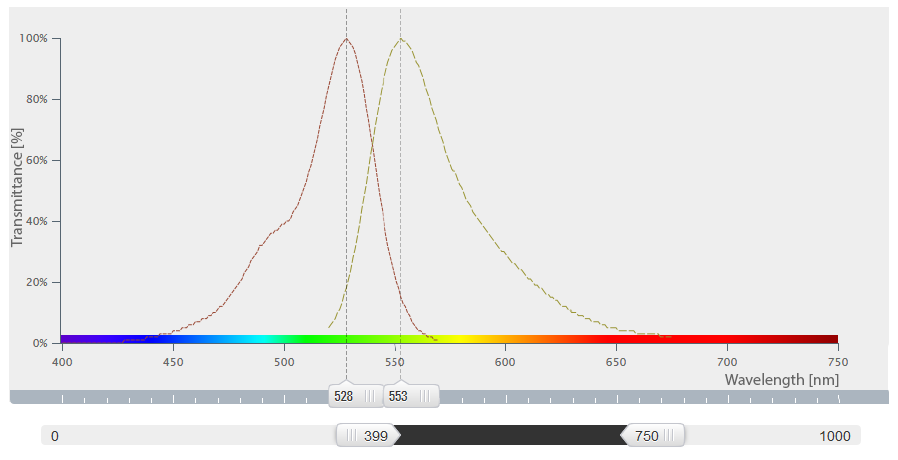
\includegraphics[width=\columnwidth]{Fluor532_ExcitationEmissionSpectrum.png}
	\caption{Normalised Excitation and Emmision Spectra of the Alexa Fluor 532 flurophore. The emmission maximum is at $553nm$ which is a more yellow-green than excitation maximum at $528nm$. This image was generated using FluoScout\texttrademark\, web application by Leica Microsystems for determining the optimal fluorescence filter cube set. %\url{http://www.leica-microsystems.com/fluoscout/}
	}
	\addloflink{http://www.leica-microsystems.com/fluoscout/}
	\label{fig:excitationandemissionspectra}
\end{figure}

\begin{figure}[!h]
	\centering
	\subfigure[]
	{
		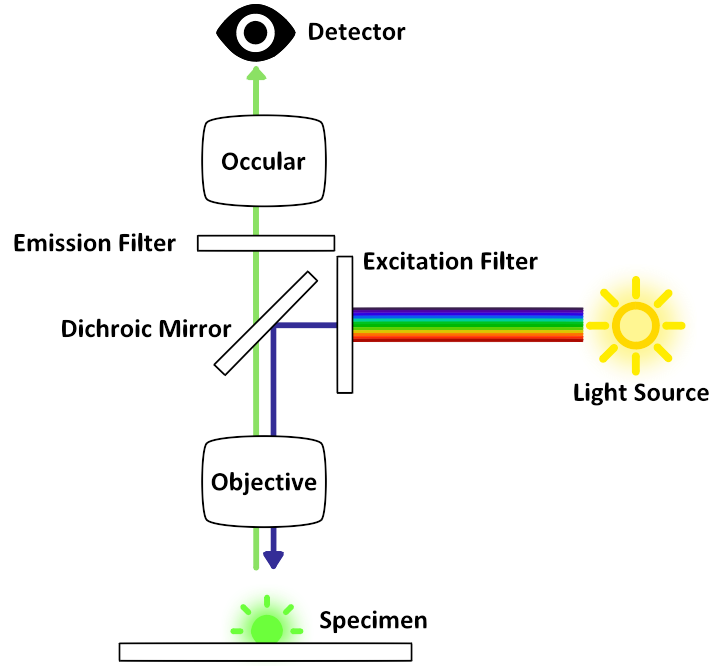
\includegraphics[width=0.36\columnwidth]{Epifluorescence_Microscope.png}
		\label{fig:epifluorescencemicroscope}
	}
	\subfigure[]
	{
		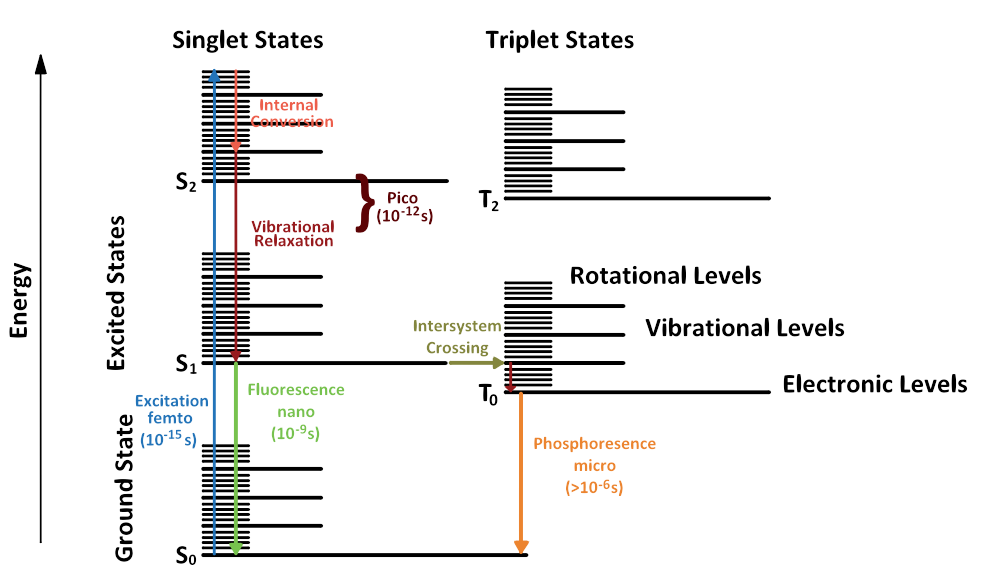
\includegraphics[width=0.60\columnwidth]{jablonski_diagram.png}
		\label{fig:jablonski}
	}
	\caption{\textbf{(a)} The schematic of the epifluorescence microscope. \textbf{(b)} The Jabloski diagram depicting the electronics states from photon absorption to photo emission.}
	\label{fig:thinkoflabel}
\end{figure}

%----------------------------------------------------------------------------------------
%	SECTION 2
%----------------------------------------------------------------------------------------

\section{Specimen Labelling}
\label{sec:SpecimenLabelling}

\textcolor{red}{Why do specimens have to be stained? What is is staining?}
Many of the components of interest, such as cell nuclei, cytoplasm, genes, chrosomes, proteins, do not possess a high degree of autofluorescence. 
In this scenario, these components can be marked with a fluorescent dye \citep{Tsien1998}, also known as a fluorophore or fluorochrome, a substance that can bind to a specific target whose excitation and emission spectra are well known. 
This is known as staining \citep{Danek2012,Hubeny2008,Dobrucki2013}. 
Once the specimen is stained it can be indirectly observed using a fluorescence microscope.

\textcolor{red}{What are the most common staining protocols?}
The most prevalent staining techniques are fluorescence in-situ hybridisation (FISH) and immunostaining \citep{Danek2012,Fatima2008,Kozubek2001_2,Theodosiou2007}.

\begin{definition}[FISH staining]
	\textcolor{red}{What is FISH?	What is the FISH staining techniques used for?}
	FISH is a molecular cytogenetic technique that uses flourophores that bind to selected regions in nucleic acids \citep{Danek2012,Fatima2008}.
	FISH is the most frequently used staining technique used primarily for visualisation and localisation of nucleic acid sequences, chromosomes, cytplasm or organelles which contain those acids \citep{Hubeny2008}.
	This makes FISH highly attractive for finding specific features in DNA and RNA used in genetic diagnosis and research, medicine and species identification \citep{Amann2008,Fatima2008}.
	Figure \ref{fig:FISH} is a capture of mouse chromosomes using the FISH staining technique.
\end{definition}

\begin{definition}[Immunostaining]
	\textcolor{red}{What is Immunofluorescence and the two main types, what is the difference between the two, and which is more common? What is the Immunofluorescence staining techniques used for?}
	Immunofluorescence is the detection method where an antibody is used to detect an antigen in a tissue or a cell using fluorescence.
	The two types of immunofluorescent detection are immunocytofluorescence (ICF) and immunohystofluorescence (IHF).
	It must not be confused with immunocytochemistry (ICC) and immunohistochemistry (IHC).
	\textit{Immuno} refers to the immunological technique, i.e. the binding of antibodies to antigens.
	\textit{Cyto} refers to cells, i.e. cells without the extracellular matrix.
	\textit{Histo} refers to tissue i.e. cells with the extracellular matrix.
	\textit{Chemistry} refers to the chemical method of detection, e.g. a change in colour.
	\textit{Fluorescence} detection by emission of light \citep{Katikireddy2011}.
	Figure \ref{fig:IHC} shows the detection of the p53 Binding Protein 1 in perfusion fixed frozen sections of rat kidney.
\end{definition}

\begin{definition}[Live-cell staining]
	\textcolor{red}{FISH and IHC cannot stain live cells. Why? How can we stain live cells?}
	The previously discussed staining techniques are not suitable to observe living cells.
	The fluorescent dyes used are phototoxic and cause cells to die. The circumvent this problem an elegant solution has been devised.
	Instead of staining, the cells are modified to produce a fluorescent substance in the target structures.
	Derivatives of the \textit{green fluorescent protein} (GFP), isolated from the \textit{Aequorea victoria} jellyfish \citep{Tsien1998,LichtmanConchello2005,Fatima2008}, are used as it generates a strong photon emission and is non-toxic to living cells \citep{Danek2012,Hubeny2008,Dobrucki2013}.
\end{definition}

%\textcolor{red}{Important notes about fluorophores and the impact on image quality?}

% IHC staining
% Marker of gene expression and protein tagging \citep{Tsien1998}\\
% Biological Fluorescence Stains, Immunofluorescence, Fluorescent Proteins\\


%\begin{figure}[!h]
%	\centering
%	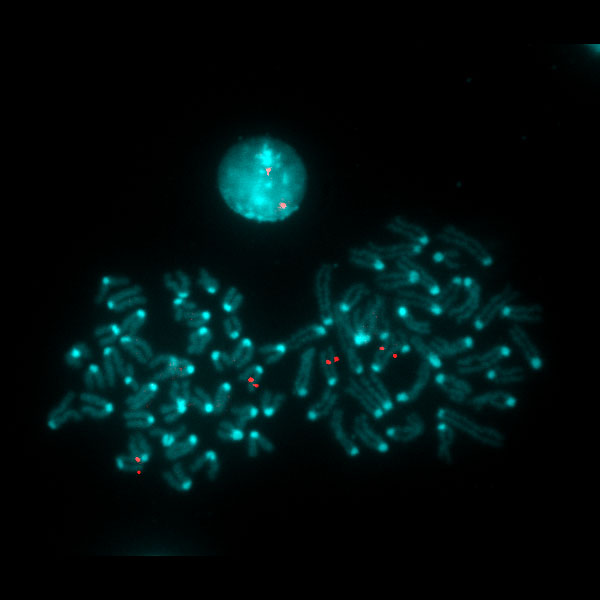
\includegraphics[width=0.5\columnwidth]{fish1.jpg}
%	\caption{FISH (Fluorescent 'in-situ' Hybridization) in mouse chromosomes using a BAC clone labeled with Spectrum Orange. The picture shows two metaphases and one interphase with two signals in each exampling a homozygous mouse for a transgenic clone. The image is taken from "All About the Human Genome Project" Genetic and Genomic Image and Illustration Database: \url{https://unlockinglifescode.org/media/images/}}
%	\label{fig:FISH}
%\end{figure}
%
%\begin{figure}[!h]
%	\centering
%	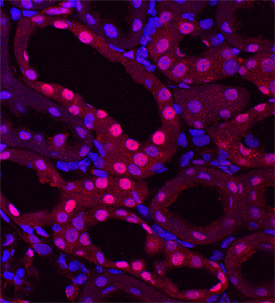
\includegraphics[width=0.5\columnwidth]{ihc1.jpg}
%	\caption{p53 Binding Protein 1 (53BP1) was detected in perfusion fixed frozen sections of rat kidney using Goat Anti-Human 53BP1 Antigen Affinity-purified Polyclonal Antibody (Catalog \# AF1877) at 15 $\mu$g/mL overnight at 4\degree C. Tissue was stained using the NorthernLights\texttrademark 557-conjugated Anti-Goat IgG Secondary Antibody (red; Catalog \# NL001) and counterstained with DAPI (blue). Specific staining was localized to nuclei of epithelial cells in convoluted tubules. The image is taken from R\&D Systems' IHC image database: \url{https://www.rndsystems.com/resources/ihc-images/53bp1}}
%	\label{fig:IHC}
%\end{figure}

\begin{figure}[!t]
	\centering
	\subfigure[]
	{
		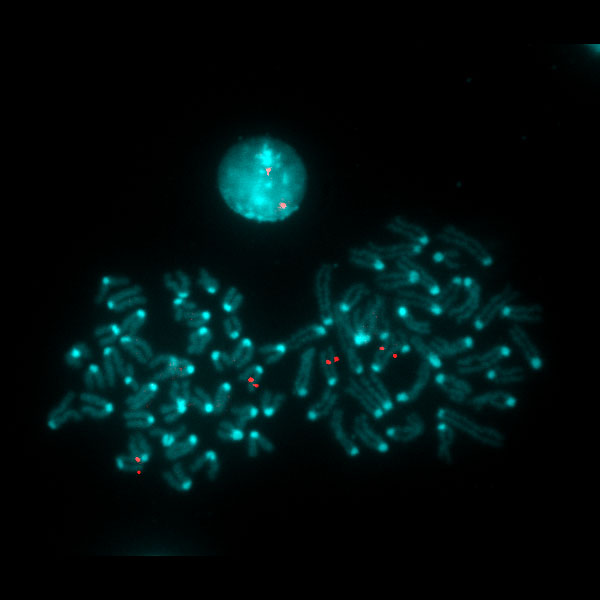
\includegraphics[width=0.495\columnwidth]{fish1.jpg}
		\label{fig:FISH}
	}
	\subfigure[]
	{
		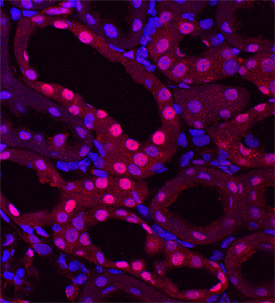
\includegraphics[width=0.45\columnwidth]{ihc1.jpg}
		\label{fig:IHC}
	}
	\caption{\textbf{(a)} FISH (Fluorescent 'in-situ' Hybridization) in mouse chromosomes using a BAC clone labeled with Spectrum Orange. The picture shows two metaphases and one interphase with two signals in each exampling a homozygous mouse for a transgenic clone. Image Source: "All About the Human Genome Project" Genetic and Genomic Image and Illustration Database. %\addloflink{https://unlockinglifescode.org/media/images/} %\url{https://unlockinglifescode.org/media/images/}. 
	\textbf{(b)} p53 Binding Protein 1 (53BP1) was detected in perfusion fixed frozen sections of rat kidney using Goat Anti-Human 53BP1 Antigen Affinity-purified Polyclonal Antibody (Catalog \# AF1877) at 15 $\mu$g/mL overnight at 4$^{\circ}$C. Tissue was stained using the NorthernLights\texttrademark 557-conjugated Anti-Goat IgG Secondary Antibody (red; Catalog \# NL001) and counterstained with DAPI (blue). Specific staining was localized to nuclei of epithelial cells in convoluted tubules. Image Source: R\&D Systems' IHC image database.}
	%\addloflink{https://www.rndsystems.com/resources/ihc-images/53bp1}}
	%\url{https://www.rndsystems.com/resources/ihc-images/53bp1}.}
	\addloflink{https://unlockinglifescode.org/media/images/}
	\addloflink{https://www.rndsystems.com/resources/ihc-images/53bp1}
	\label{fig:stainingtechniques}
\end{figure}

%----------------------------------------------------------------------------------------
%	SECTION 3
%----------------------------------------------------------------------------------------

\section{The Epifluorescence Microscope and Image Acquisition}
\label{sec:TheEpifluorescenceMicroscope}

Schematic layout of a Fluorescence Microscope. Process, function of each component\\
Other Types of Fluorescence Microscopes: Confocal, TIRF, Epifluorescence\\
Acquisition: CCD\\
Hardware setup effect on image quality.\\
Numerical Aperture, Sub-diffraction\\

%----------------------------------------------------------------------------------------
%	SECTION 4
%----------------------------------------------------------------------------------------

\section{Image Processing in FM}
\label{sec:ImageProcessingInFM}

Limitations in Fluorescence Imaging\\
Preprocessing: Point Spread Function deconvolution, etc\\
Segmentation 

%----------------------------------------------------------------------------------------
%	SECTION 5
%----------------------------------------------------------------------------------------

\section{Measurements and Analysis in FM}
\label{sec:Measurements}

what is measured and for what?\\
Motion, number of cells, area, volume, lenght